\section*{Figures}

\begin{figure}[t]
\centering
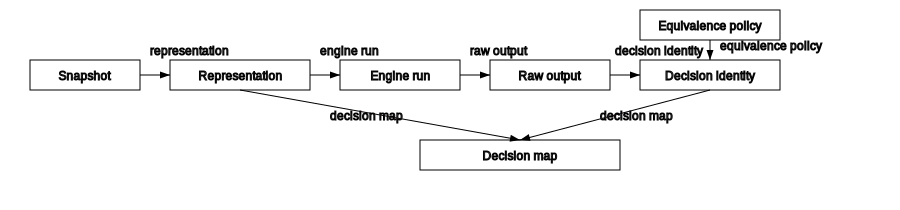
\includegraphics[width=\linewidth]{../../2026-01-31/agents/work-tree/figures/figure1_canonical_schematic.pdf}
\caption{Canonical decision-valued mapping schematic. A fixed snapshot is encoded into a representation family. Each representation is executed by a fixed engine and yields raw output. An equivalence policy extracts a discrete decision identity from the raw output. The decision map links representation identifiers, engine runs, and decision identities.}
\label{fig:canonical-decision-map}
\end{figure}

\begin{figure}[t]
\centering
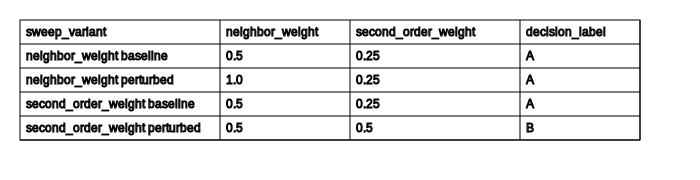
\includegraphics[width=\linewidth]{../../2026-01-31/agents/work-tree/figures/figure2_primary_sweep.pdf}
\caption{Primary representational sweep for one snapshot and engine. Each variant corresponds to a weight setting recorded in the weight variation results. Decision identity is defined by the route node sequence in each variant. Identical identities use the same label.}
\label{fig:primary-representational-sweep}
\end{figure}

\begin{figure}[t]
\centering
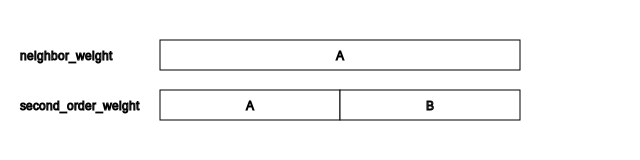
\includegraphics[width=\linewidth]{../../2026-01-31/agents/work-tree/figures/figure3_identity_persistence.pdf}
\caption{Identity persistence regions derived from Figure 2. Consecutive variants with identical decision identity labels are shown as a single region, indicating persistence under the tested weight changes.}
\label{fig:identity-persistence}
\end{figure}

\begin{figure}[t]
\centering
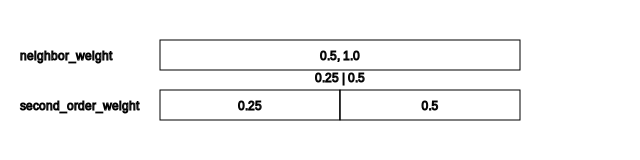
\includegraphics[width=\linewidth]{../../2026-01-31/agents/work-tree/figures/figure4_boundary_fracture.pdf}
\caption{Boundary and fracture localization derived from Figure 2. Transitions where route\_changed or edge\_order\_changed is true are marked as boundaries, with baseline and perturbed weight values listed.}
\label{fig:boundary-fracture}
\end{figure}

\begin{figure}[t]
\centering
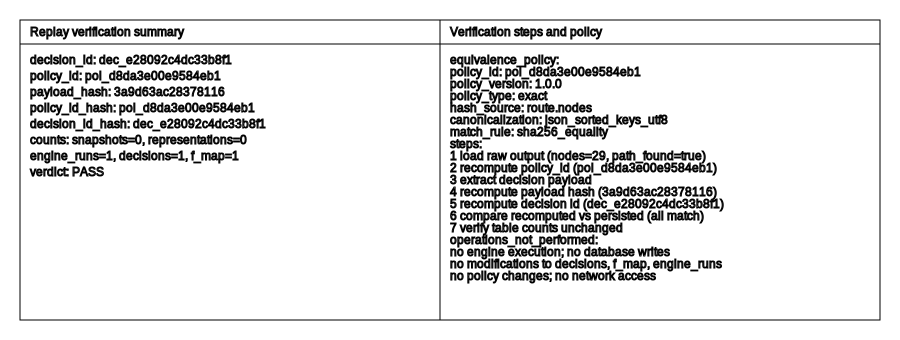
\includegraphics[width=\linewidth]{../../2026-01-31/agents/work-tree/figures/figure5_replay_verification.pdf}
\caption{Reproducibility replay verification. The replay verification logs show recomputed policy identifier, payload hash, and decision identifier matching the persisted manifest, and table counts remain unchanged.}
\label{fig:replay-verification}
\end{figure}

All figures will use the canonical caption template defined at the end of this manuscript. No figure will introduce performance metrics, optimization criteria, or learning claims.
